% !TEX TS-program = pdflatex
% !TEX encoding = UTF-8 Unicode
% !TEX ROOT = main.tex

\section*{Begrüßung der Orga}
Liebe ZaPFika,\\

\noindent wisst ihr, was das größte Problem bei einer ZaPF ist? -- Die ZaPFika.

Bevor die Zapfika ankommen, ist die ganze ZaPF schön. Man macht Raumpläne und Zeitpläne und AK-Pläne und Pläne, die nicht mal eigene Namen haben. Und man denkt sich Akronyme aus, man malt Logos, man schreibt lustige Texte, man denkt sich Easter Eggs aus und erzählt natürlich der ganzen Welt, was für eine tolle ZaPF man macht. Die ganze ZaPF ist nur auf Papier und unseren Festplatten, es tauchen keine Probleme auf, alles ist ordentlich, organisiert und übersichtlich. Und natürlich ist es bis jetzt billiger. Wirklich viel billiger.

Dann kommen die ZaPFika. Und \textit{aaahhh!!!} überall Menschen und sie tun dumme Dinge und sie haben Gepäck, so viel Gepäck, überall Gepäck und Autos, Autos müssen irgendwo parken, warum haben wir da nicht dran gedacht, warum haben wir uns da nicht drum gekümmert, aber die Autos müssen jetzt weg weg weg WEG!!! und die ZaPFika wollen was zu essen und das Chili ist zu scharf und das Chili ist nicht scharf genug und jetzt wollen sie ins Anfangsplenum, aber die Plenums-Technik funktioniert nicht und warum funktioniert sie nicht, gestern ging doch alles noch und die ZaPFika werden ungeduldig und wissen nicht, was sie tun sollen, und tun einfach irgendwas und sie beschweren sich die ganze Zeit und endlich geht das Anfangsplenum los und warum wollen sich denn jetzt noch Leute anmelden und wo sind die Anmeldungshelfika hin und wo sind die Listen hin und warum gibt es keine Tagungstaschen mehr und \dots wie können nur 200 ZaPFika eigentlich so viel Dreck machen\dots\textit{Und das ist nur der erste Tag.}

Nun gut, irgendwann sind die ZaPFika dann wieder weg. Jetzt müssen wir nur noch den ganzen Müll wieder aufräumen, den Schaden am Inventar verbergen, die Leichen aus den Seminarräumen holen bevor der Lehrbetrieb weitergeht, den Hausmeister, den Institutsleiter und den Dekan besänftigen und alles zurücknehmen, was wir unserer Fachschaft gegenüber im Zorn gesagt haben. Und dann, wenn alle Spuren der ZaPFika getilgt sind und wieder himmlische, akademische Ruhe in unseren Hallen eingekehrt ist, setzen wir uns gemütlich daran, den Reader zu schreiben. Und dann ist die ZaPF wieder nur auf Papier, ohne Probleme, ohne Chaos, ergebnisorientiert in Reih und Glied, so wie es sein sollte.

\begin{wrapfigure}{r}{6cm}
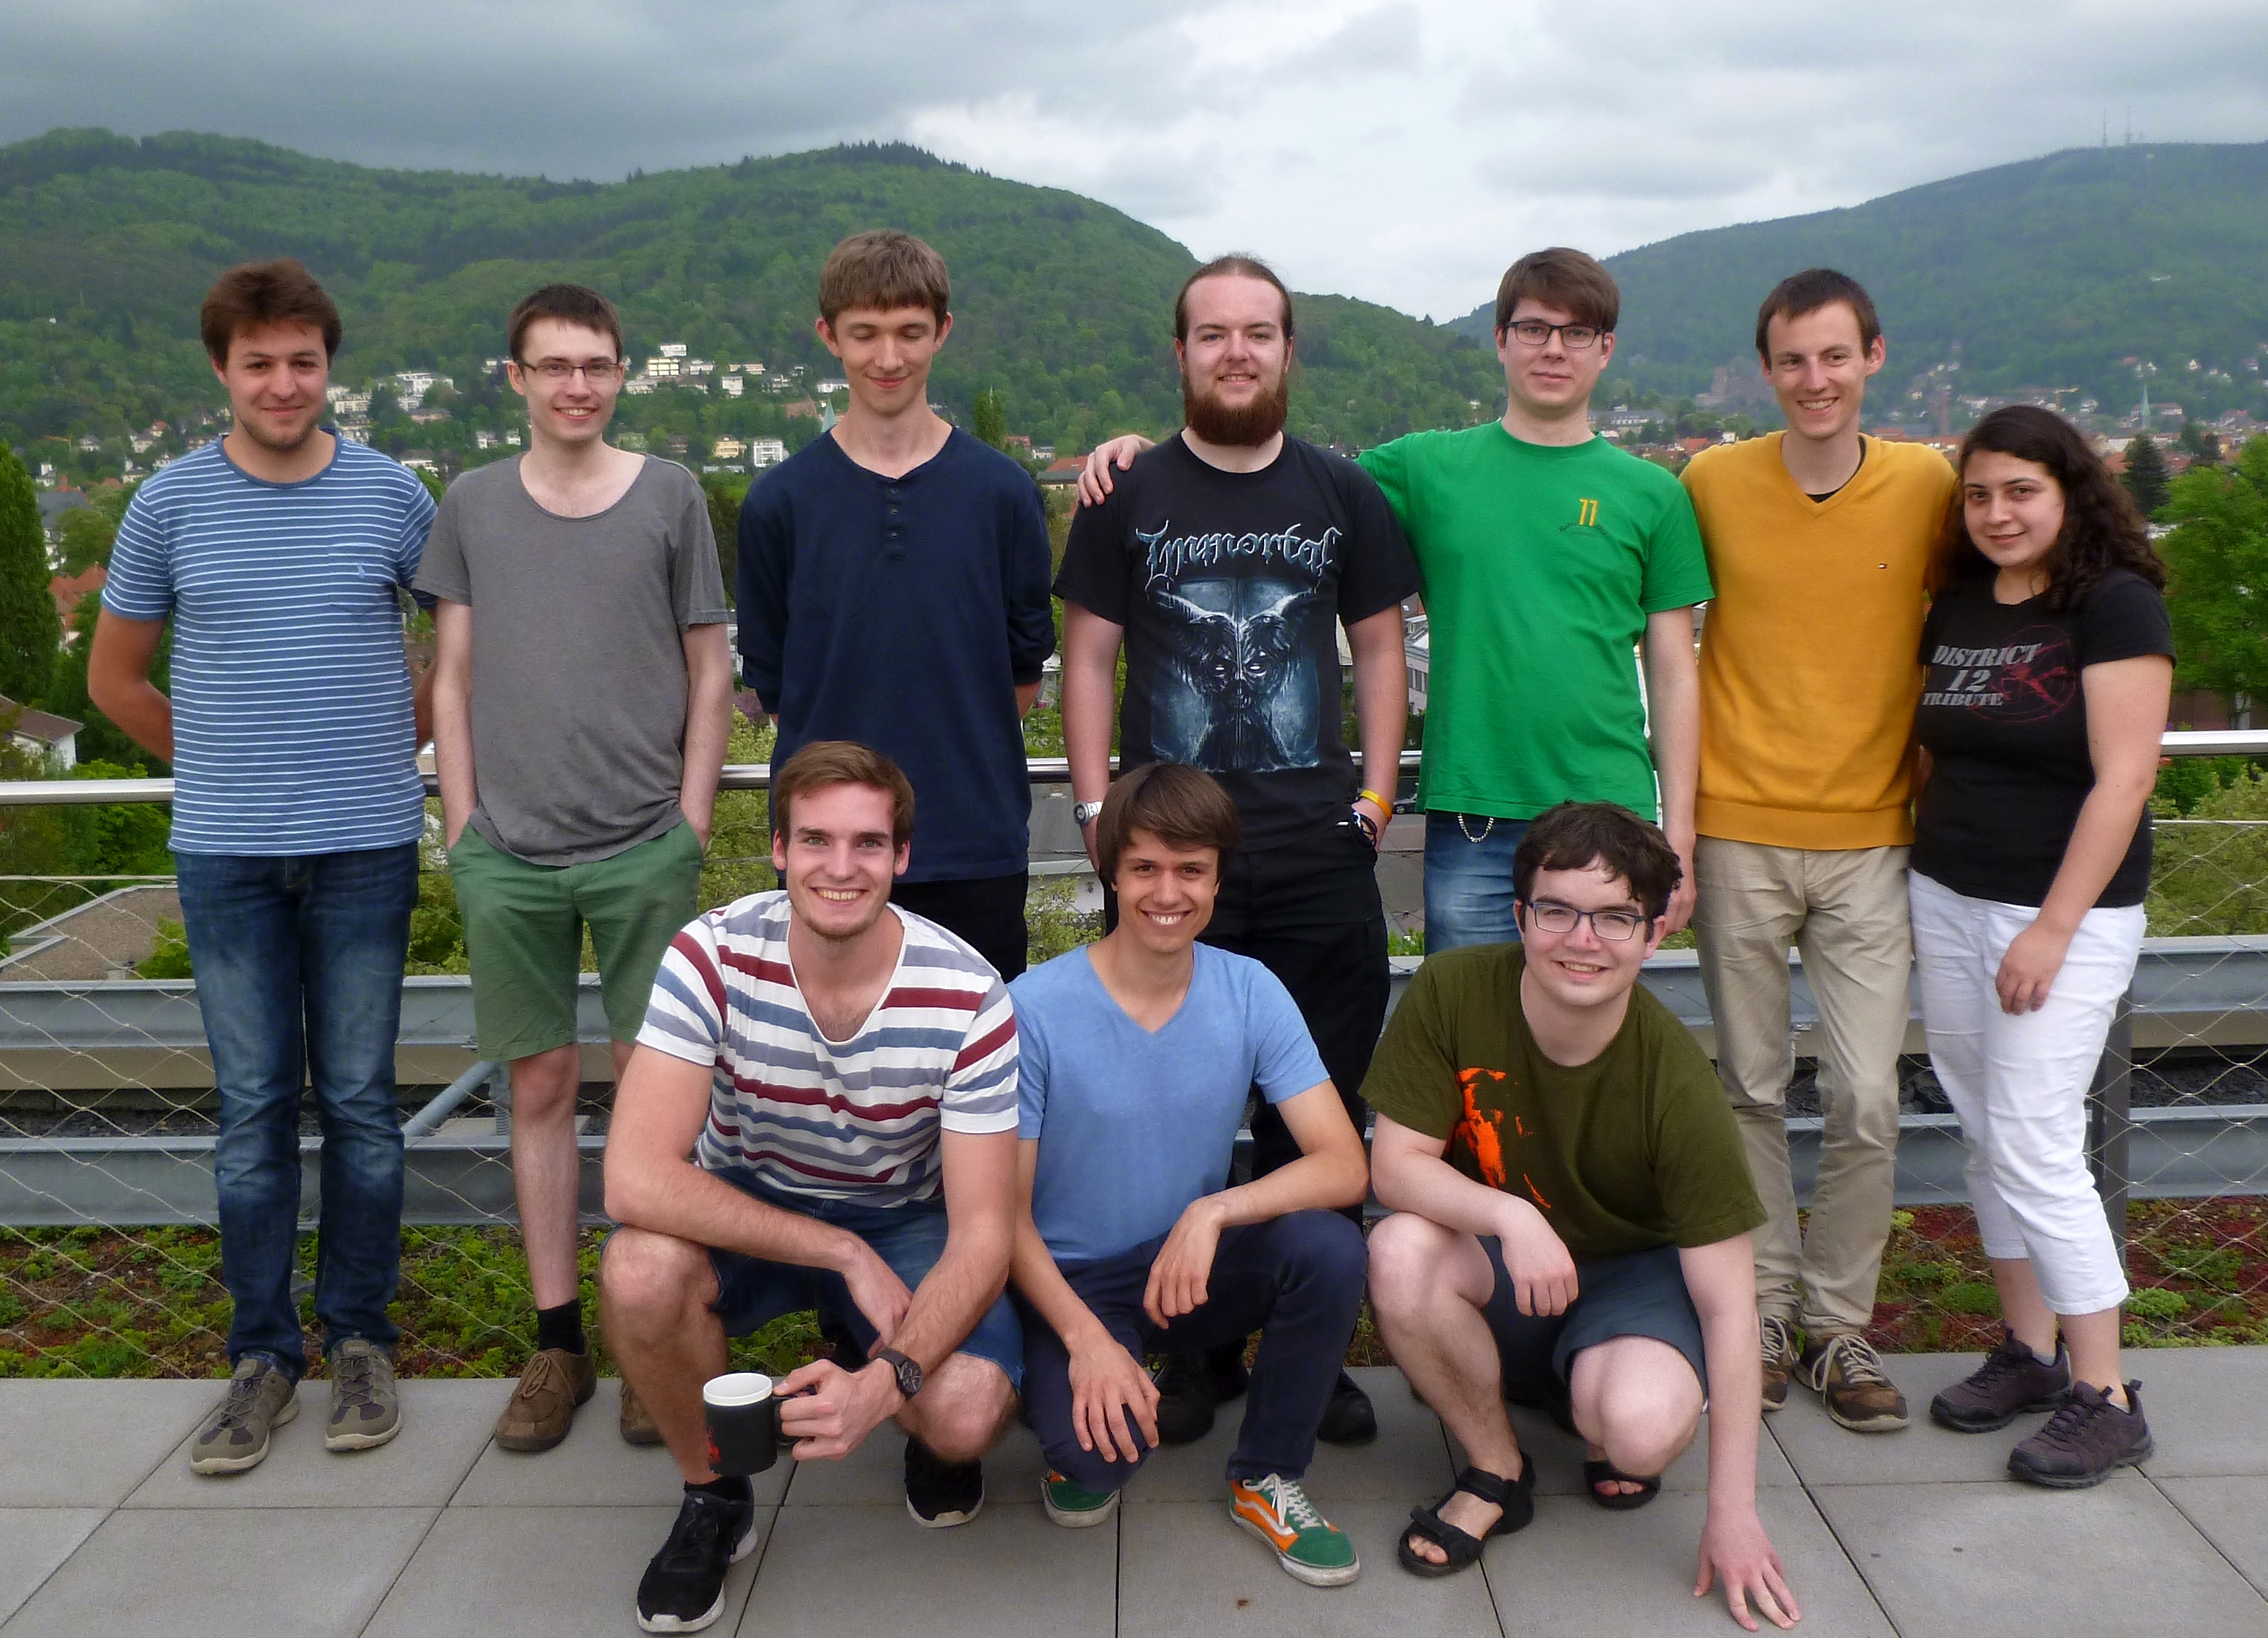
\includegraphics[width=.65\textwidth]{media/orga}
\end{wrapfigure}

Andererseits studieren wir Physik\footnote{Außer die ganzen Mathematika und Informatika in unserem Orga-Team natürlich. Die studieren Mathematik oder Informatik.} und treiben uns in einer Fachschaft rum. Also haben wir offensichtlich Spaß an Problemen. Und wir kennen kein tolleres, lustigeres oder absurderes Problem in 200 einzigartigen Ausführungen als euch.

Wir hoffen natürlich, dass es euch auf unserer ZaPF und hier in Heidelberg so gut gefällt, dass ihr direkt hierbleibt und einfach eine 200 PhysikerInnen starke WG unter der Ernst-Walz-Brücke aufmacht.

Zu den technischen Aspekten der ZaPF: Solltet ihr in diesem Heft auf der Suche nach Antworten auf die wirklich relevanten Fragen\footnote{Gibt es auch Alternativen dazu, unter der Brücke zu schlafen? Wie ging dieses Lied mit der Ente, Ente nochmal?} sein, werdet ihr auf allen anderen Seiten des Tagungshefts auch fündig werden. Und falls euch nach der Lektüre immer noch etwas auf dem Herzen liegt, kommt einfach auf uns zu. Ok, das wars mit den technischen Aspekten, es wünscht euch\\

Viel Spaß und eine schöne ZaPF

eure Heidelberger ZaPF-Orga
